\documentclass[titlepage, a4paper,12pt]{article}

\usepackage[T2A]{fontenc}	
\usepackage[utf8]{inputenc}	
\usepackage[english,russian]{babel}
\usepackage{amsmath,amsfonts,amssymb,amsthm,mathtools} 
\usepackage[pdftex]{graphicx}
\graphicspath{{images/}}
\usepackage{wrapfig}
\usepackage{wasysym}
\usepackage{textcomp}
\usepackage{indentfirst}
\usepackage{amsmath}
\usepackage[colorlinks,urlcolor=blue]{hyperref} %ссылки
\usepackage{titlepic}

\author{Легошин Алексей (Б02-924), Привалов Андрей (Б02-922)}
\title{
Горизонты физики. \\
Введение в волновую оптику.
}
\date{\today}
\titlepic{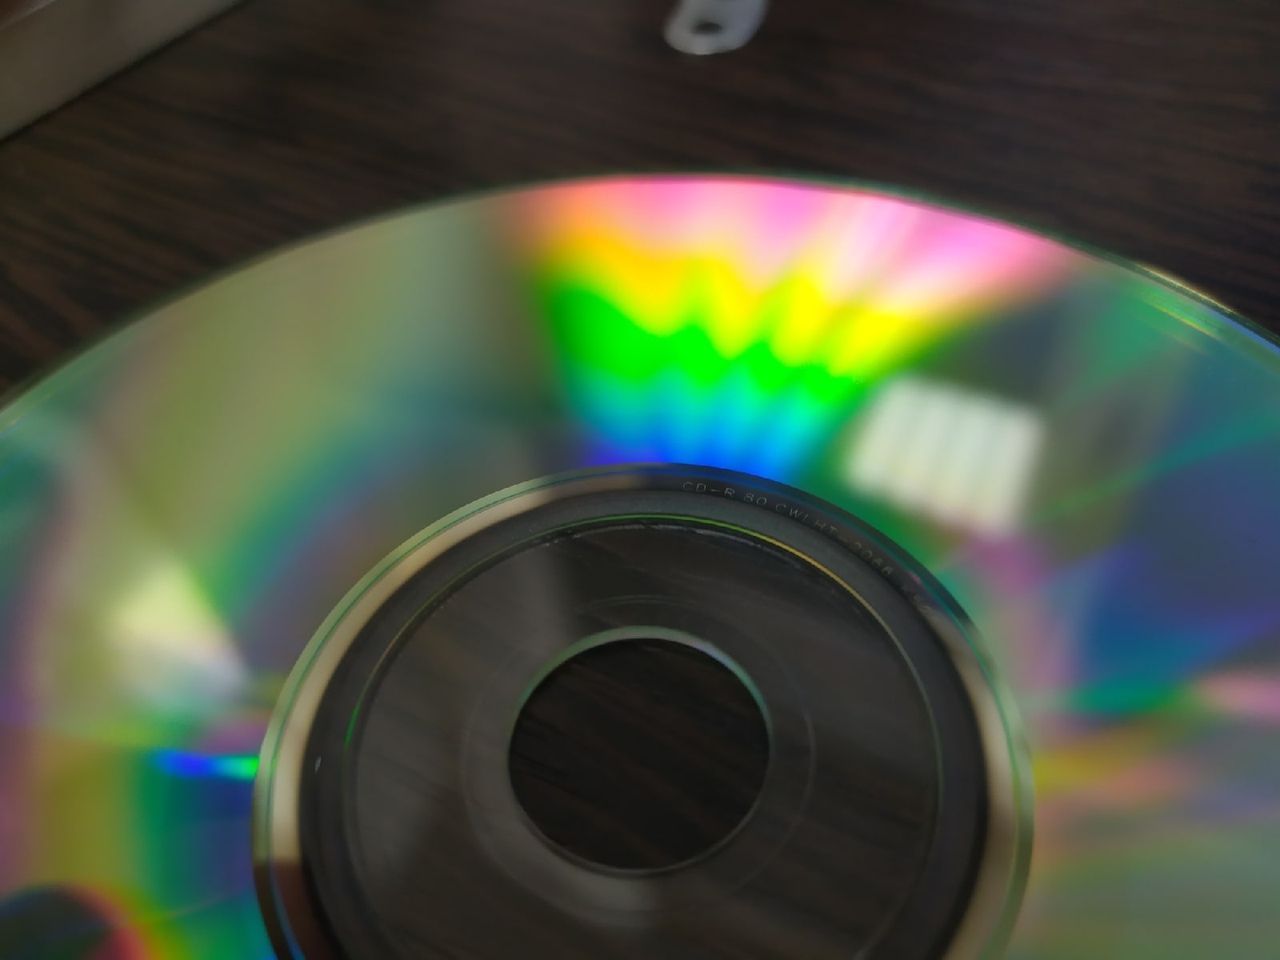
\includegraphics[width=8cm]{title}}



\begin{document}

	\maketitle

	\newpage
	
	\section{Ход работы}
	
	Настроили установку.
	
	\begin{figure}[h!]
		\begin{center}
			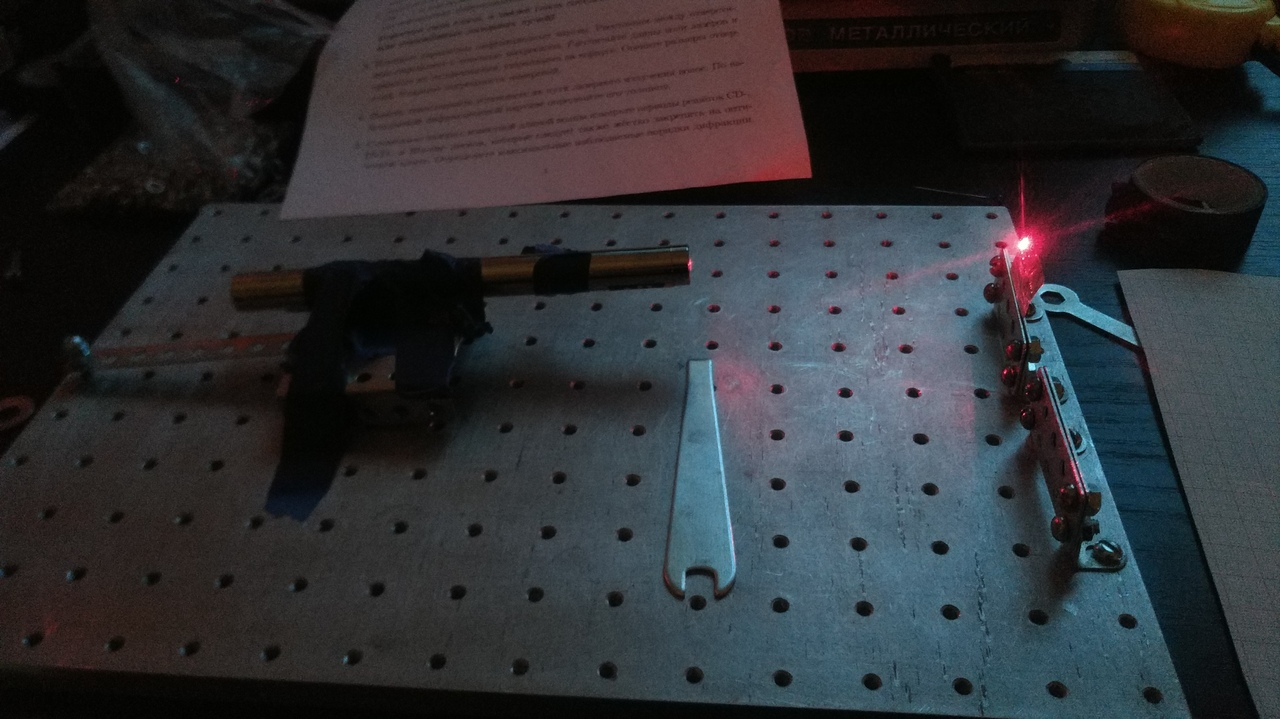
\includegraphics[width = 0.95\textwidth]{1}
			\caption{Собранная установка}
			\label{ris:1}
		\end{center}
	\end{figure}
	
	\subsection{Определение расстояния между щелями при помощи дифракции}
	
	С красным лазером на расстоянии 9,5 см от щели и расстоянием между щелью и экраном 159 см наблюдали кольца при двух разных расстояниях между отверстиями. В первом случае расстояние между дифракционными полосами составило $\approx$ 3 мм, во втором --- $\approx$ 0.5 мм.
	
		\begin{figure}[h!]
		\begin{center}
			\begin{minipage}[h]{0.49\linewidth}
				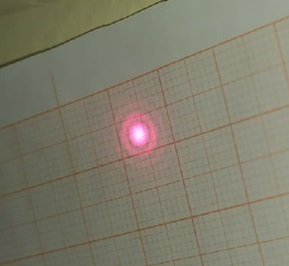
\includegraphics[width=1\linewidth]{2_1}
				\caption{Дифракция для более частой решётки} %% подпись к рисунку
				\label{ris:2.1} %% метка рисунка для ссылки на него
			\end{minipage}
		\hfill
			\begin{minipage}[h]{0.49\linewidth}
				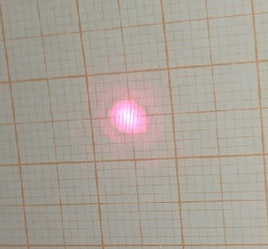
\includegraphics[width=1\linewidth]{2_2}
				\caption{Дифракция для редкой решётки}
				\label{ris:2.2}
			\end{minipage}
		\end{center}
	\end{figure}
	
	$$ d = \frac{\lambda l}{x}, $$
	$x$ -- расстояние между кольцами, $\lambda$ -- длина волны, $l$ -- расстояние от щелей до экрана.
	
	Для первой решётки: \\
	$$ d_1 = \frac{0.4 \cdot 10^{-6} \cdot 1.6}{3 \cdot 10^{-3}} = 0.23 \; mm $$
	
	Для второй решётки: \\
	$$ d_2 = \frac{0.4 \cdot 10^{-6} \cdot 1.6}{0.5 \cdot 10^{-3}} = 1.4 \; mm $$
	
	
	Измерим также расстояние между щелями при помощи микроскопа:\\
	Среднее расстояние между отверстиями более частой решётки 0.255 мм, \\
	более редкой --- 1.48 мм.
	
	Убеждаемся в неплохой точности метода измерения расстояния между щелями при помощи дифракции.
	
	\subsection{Определение толщины волоса при помощи дифракции}
	
	Поместим перед лучом лазера волос. Анализируя дифракционную картину, найдём его толщину.
	
	$$ d_h = \frac{0.4 \cdot 10^{-6} \cdot 1.6}{8 \cdot 10^{-3}} = 0.08 \; mm  $$
	При характерной толщине от 0.05 мм и до более чем 0.07, а также с учётом жёсткости измеряемого волоса, приходим к выводу, что результат получен довольно точно.
	
	\begin{figure}[h!]
		\begin{center}
			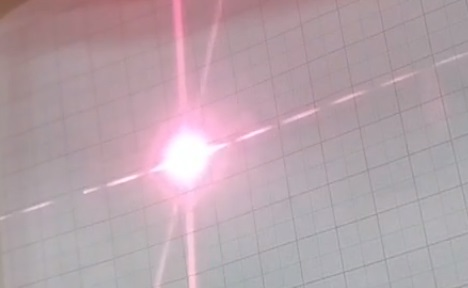
\includegraphics[width = 0.5\textwidth]{3}
			\caption{Дифракция для волоса}
			\label{ris:3}
		\end{center}
	\end{figure}
	
	\subsection{Определение решётки DVD-диска}
	
	$$ d_{DVD} = \frac{k \lambda}{\sin\varphi - \sin\theta} = \frac{2 \cdot 0.4 \cdot 10^{-6}}{0.45} \approx 1.8 \; \mu m $$
	
	\begin{figure}[h!]
		\begin{center}
			\begin{minipage}[h]{0.49\linewidth}
				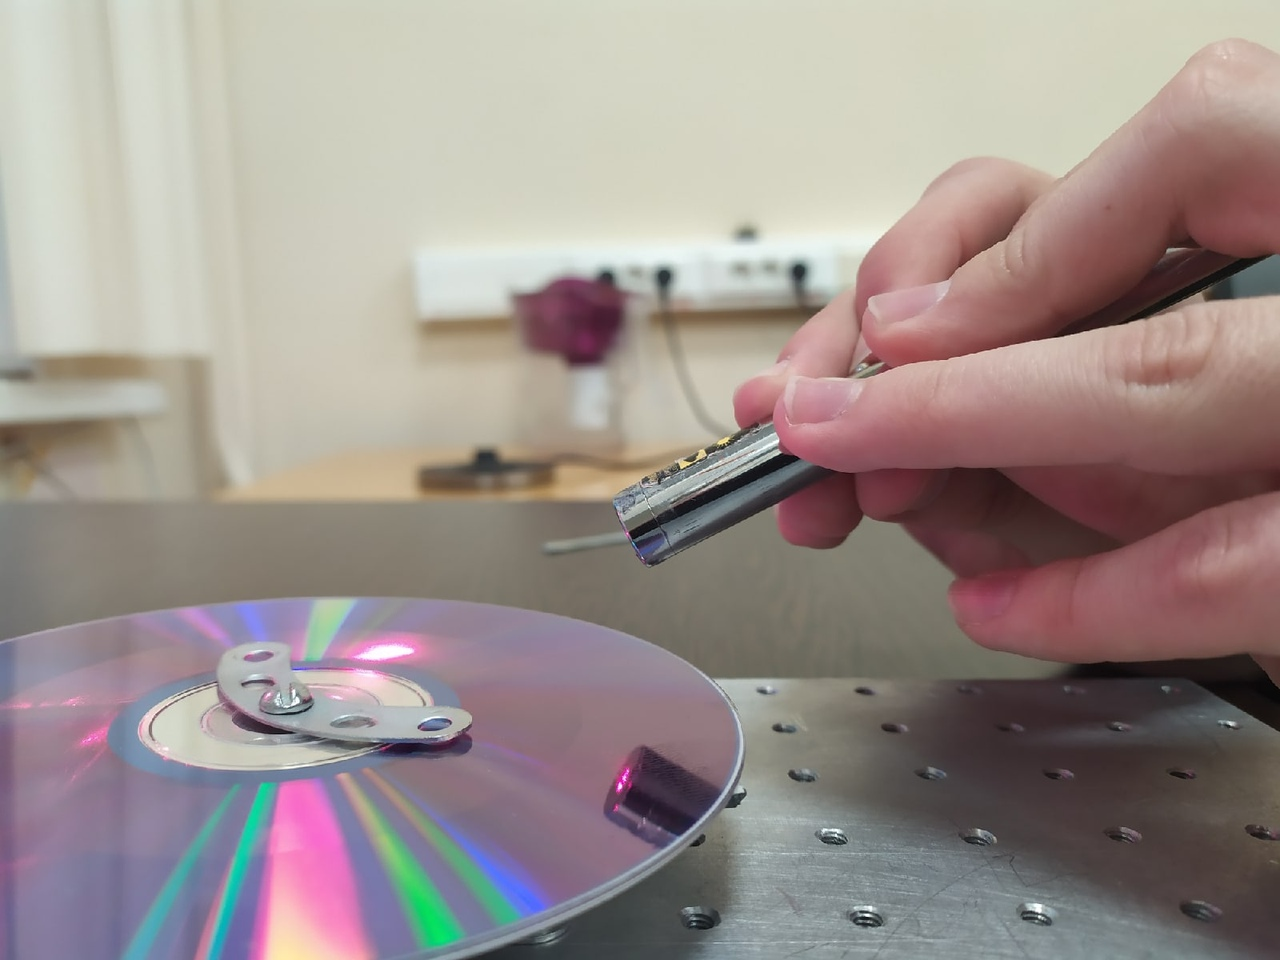
\includegraphics[width=1\linewidth]{4_1}
				\label{ris:4.1} %% метка рисунка для ссылки на него
			\end{minipage}
		\hfill
			\begin{minipage}[h]{0.49\linewidth}
				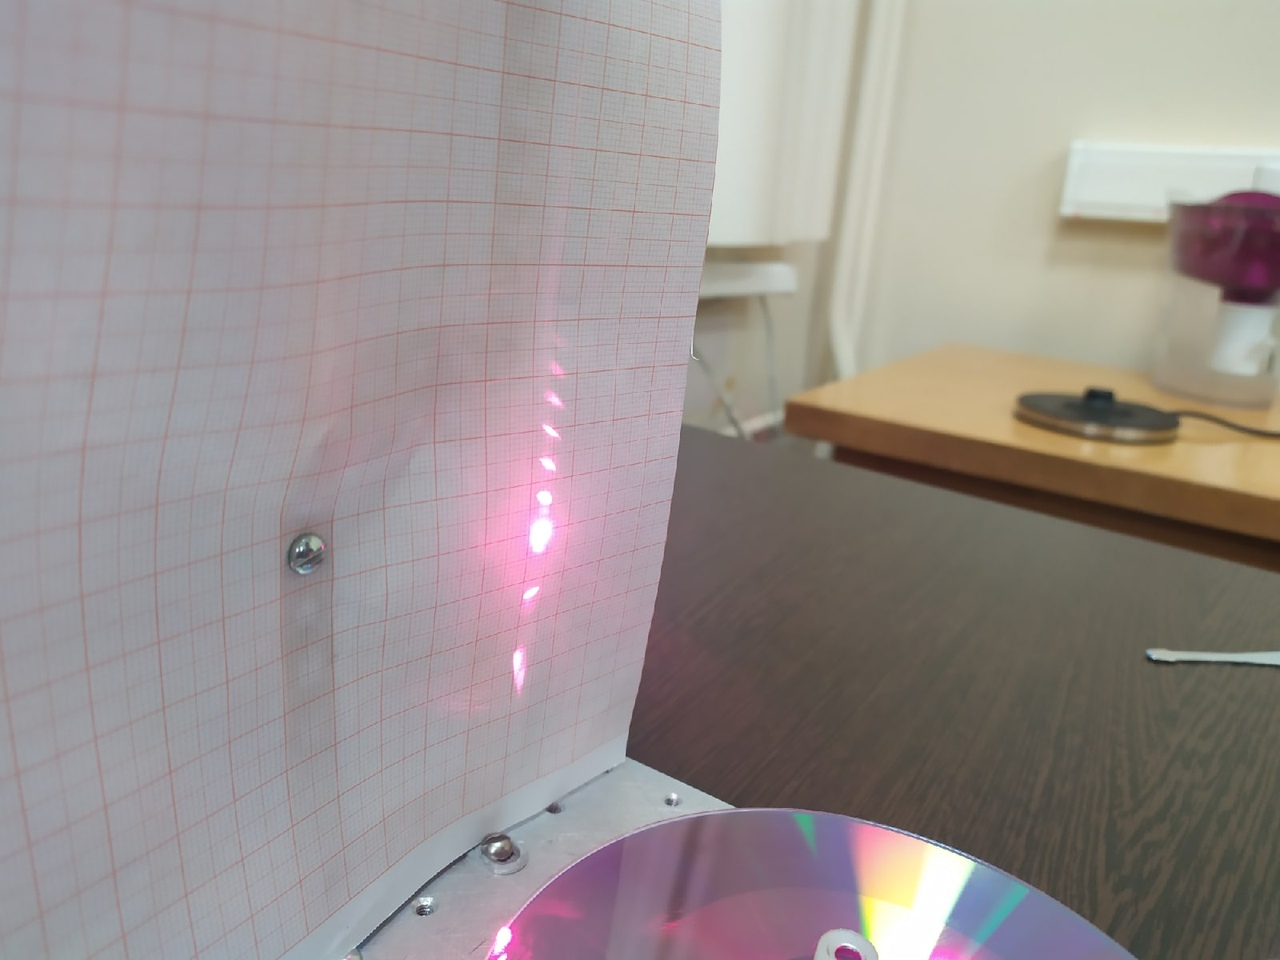
\includegraphics[width=1\linewidth]{4_2}
				\label{ris:4.2}
			\end{minipage}
			\caption{Дифракция для DVD-диска}
		\end{center}
	\end{figure}
	
	Табличное значение --- 1.6 мкм для DVD. Вновь получаем довольно точное значение.
	
	\subsection{Определение решётки CD-диска}
	
	$$ d_{CD} = \frac{k \lambda}{\sin\varphi - \sin\theta} = \frac{ 0.4 \cdot 10^{-6}}{0.71 - 0.34} \approx 1.1 \; \mu m $$
	
	\begin{figure}[h!]
		\begin{center}
			\begin{minipage}[h]{0.49\linewidth}
				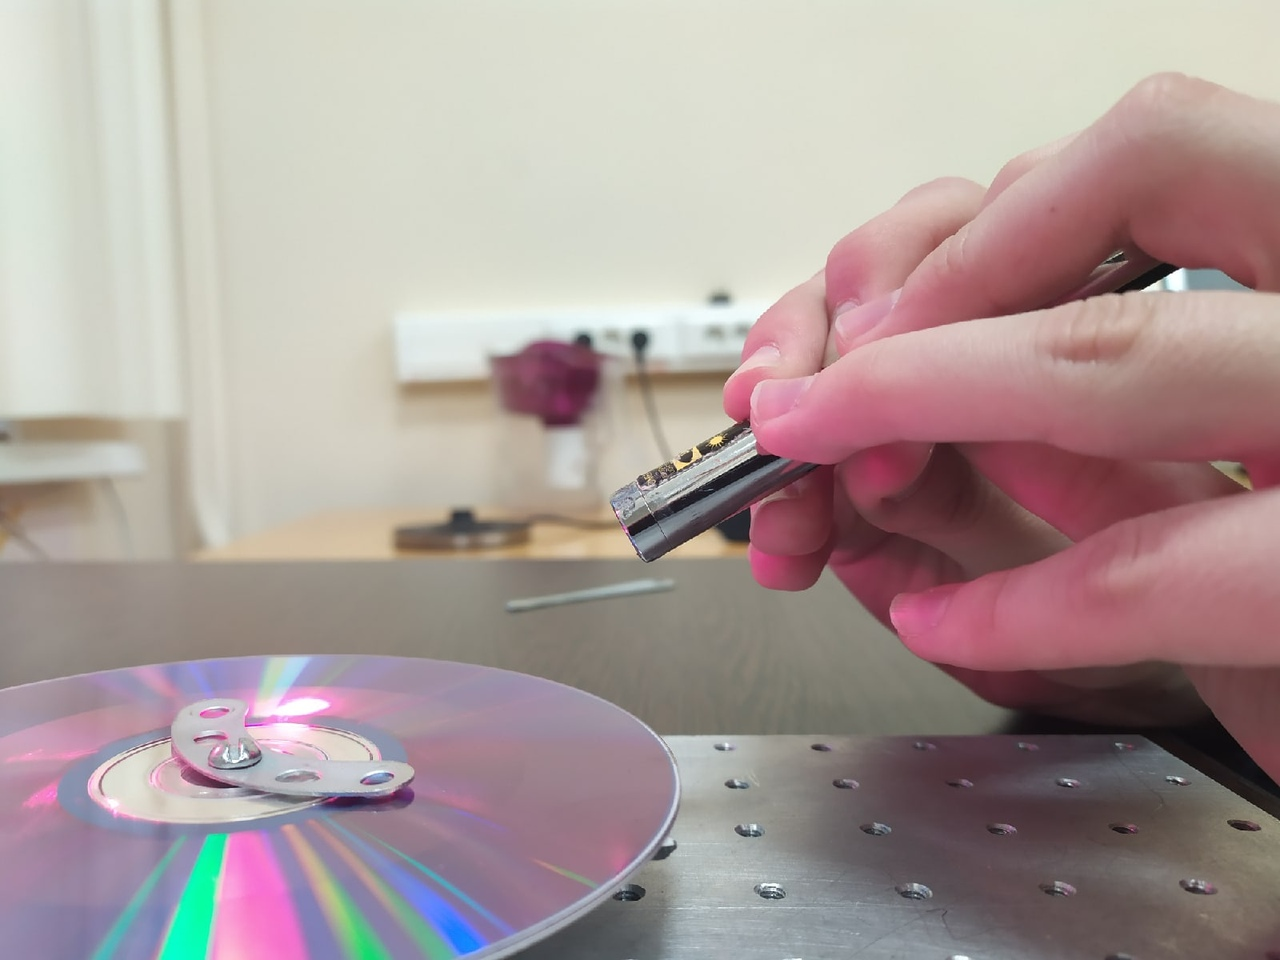
\includegraphics[width=1\linewidth]{5_1}
				\label{ris:5.1} %% метка рисунка для ссылки на него
			\end{minipage}
		\hfill
			\begin{minipage}[h]{0.49\linewidth}
				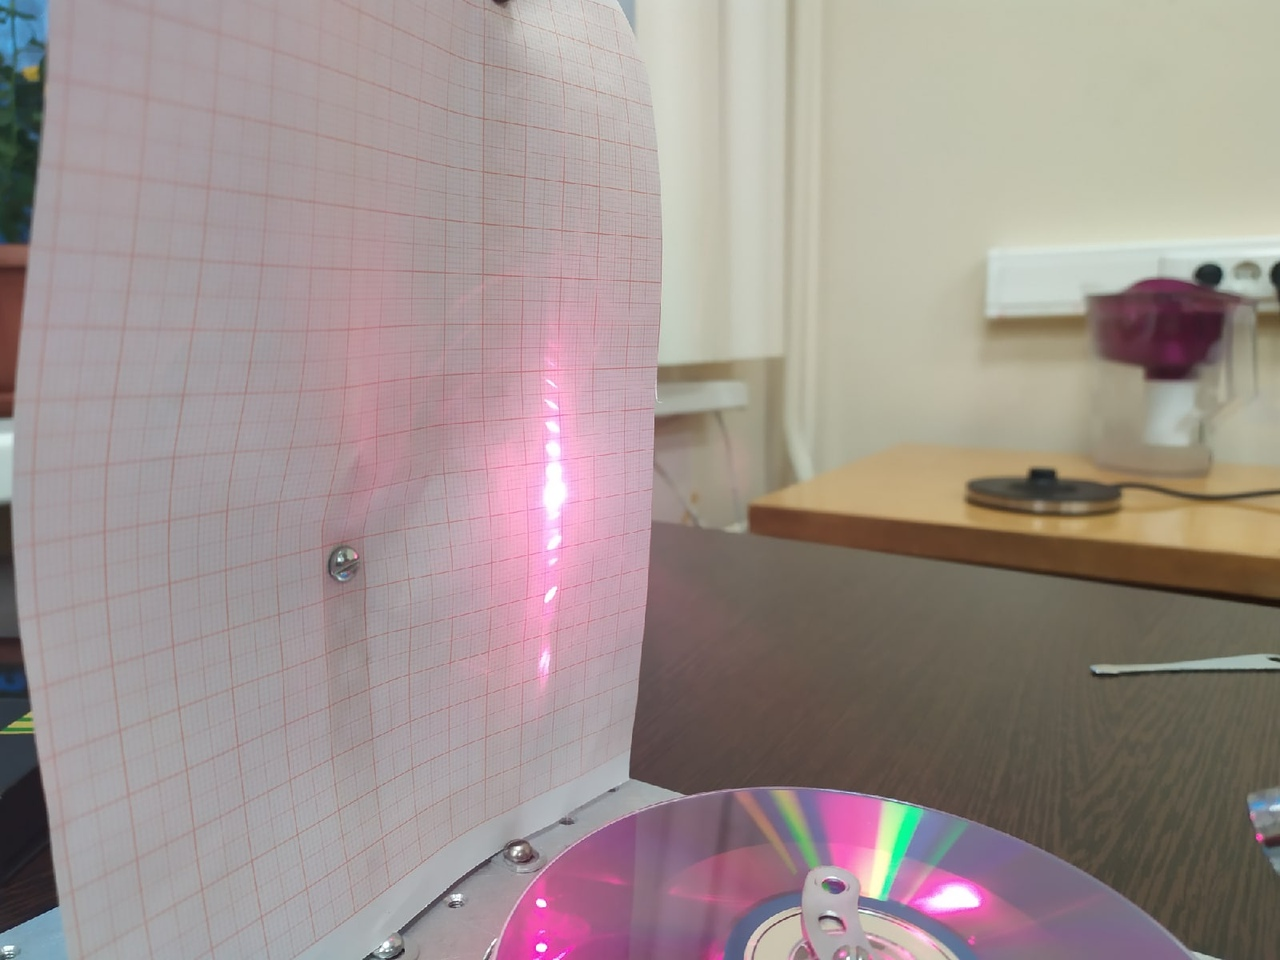
\includegraphics[width=1\linewidth]{5_2}
				\label{ris:5.2}
			\end{minipage}
			\caption{Дифракция для CD-диска}
		\end{center}
	\end{figure}
	
	Табличное значение --- 0.8 мкм для CD. Не сказать, что результат точен. Но в 0.4 мы попали.
	
		\subsection{Определение решётки Blu-Ray диска}
	
	$$ d_{CD} = \frac{k \lambda}{\sin\varphi - \sin\theta} = \frac{ 0.03 \cdot 10^{-6}}{0.225 - 0.087} \approx 0.22 \; \mu m $$
	
	\begin{figure}[h!]
		\begin{center}
			\begin{minipage}[h]{0.49\linewidth}
				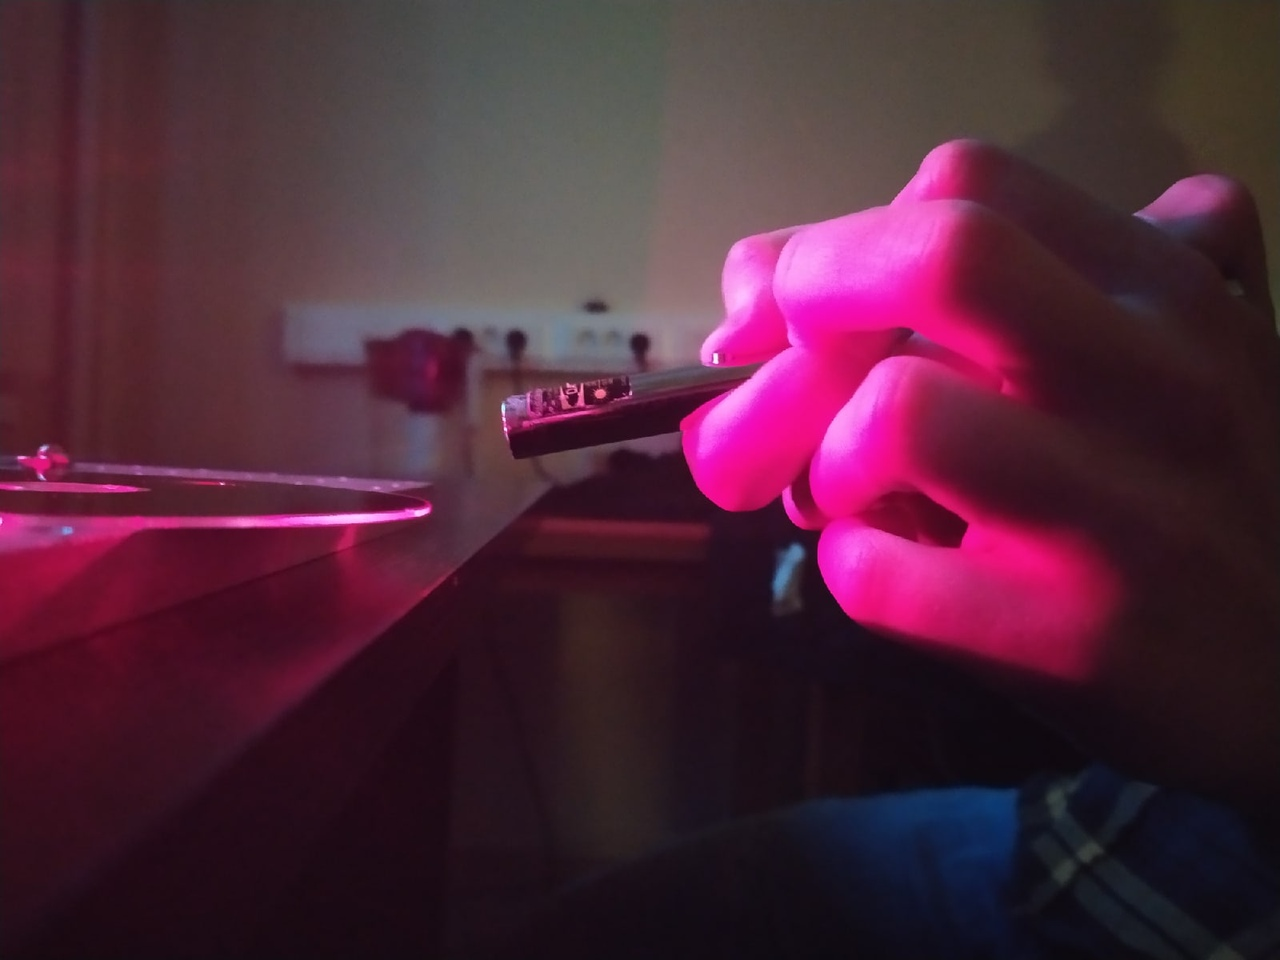
\includegraphics[width=1\linewidth]{6_1}
				\label{ris:6.1} %% метка рисунка для ссылки на него
			\end{minipage}
		\hfill
			\begin{minipage}[h]{0.49\linewidth}
				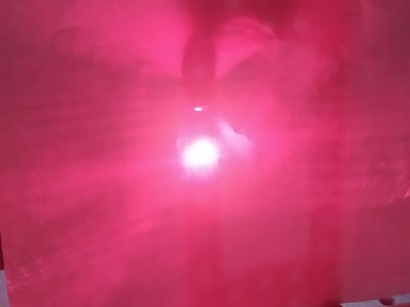
\includegraphics[width=1\linewidth]{6_2}
				\label{ris:6.2}
			\end{minipage}
			\caption{Дифракция для Blu-Ray диска}
		\end{center}
	\end{figure}
	
	Табличное значение --- 0.32 мкм для DVD. В 0.5 попали. На том спасибо.
	
	\section{Итоги}
	
	Несмотря на то, что был введён режим самоизоляции, не позволивший продолжить работу, практические задачи удалось выполнить почти полностью и получить вменяемый результат.
	
	PS: Данный документ не претендует на отчётность. Лишь обыкновенные заметки по ходу выполнения.
	
\end{document}